\lab{The Shooting Method for Boundary Value Problems}{The Shooting Method for Boundary Value Problems}
\label{lab:Shooting}
\labdependencies{IVPBVPIntro}

Consider a boundary value problem of the form
\begin{align}
	\label{eq:shooting:shooting_bvp}
	\begin{split}
y'' &= f(x,y,y'), \quad a \leq x \leq b, \\
y(a) &= \alpha, \quad y(b) = \beta.
\end{split}
\end{align}
One natural way to approach this problem is to study the initial value problem (IVP) associated with this differential equation:
\begin{align}
	\label{eq:shooting:shooting_ivp}
	\begin{split}
y'' &= f(x,y,y'), \quad a \leq x \leq b, \\
y(a) &= \alpha, \quad y'(a) = s.
	\end{split}
\end{align}
The goal is to determine an appropriate value $s$ so that the solution of the IVP \eqref{eq:shooting:shooting_ivp} is also a solution of the BVP \eqref{eq:shooting:shooting_bvp}.

Note that we can consider the value \(y(x)\) for a given initial condition \(y'(a)=s\) as a function of both \(x\) and \(s\).
Let $y(x,s)$ be the solution of \eqref{eq:shooting:shooting_ivp}.
The initial value conditions are then
\begin{align}
y(a, s) = \alpha, \quad \frac{\partial y}{\partial x}(a, s) = s.
\end{align}

We wish to find a value of $s$ so that $y(b,s) = \beta$.
Consider the function \(h(s)=y(b,s)-\beta\); this function is called the \textit{residual function}.
If \(h(s)=0\), then \(y(b,s)=\beta\) and the boundary condition is satisfied, so zeros of the function \(h\) correspond to initial conditions that are solutions to the BVP \eqref{eq:shooting:shooting_bvp}.
Applying Newton's method to the function $h(s)$, we obtain the iterative method
\begin{align*}
	s_{n+1} &= s_n - \frac{ h(s_n)}{h'(s_n) }, \\
	&= s_n - \frac{ y(b,s_n) - \beta}{\frac{\partial}{\partial s}\, y(b,s)\big|_{s_n} },\quad n = 0,1,\ldots .
\end{align*}
Provided our initial guess \(s_0\) is sufficiently good, this will converge to a value of \(s\) such that the initial value problem is also a solution to the boundary value problem.
Notice that finding $y(b,s_n)$ requires solving the initial value problem using RK4 or some other method.

We recall that Newton's method generally requires a good initial guess $s_0$.
A plausible initial guess for this setup would be the average rate of change of the solution across the entire interval, which gives $s_0 =  (\beta - \alpha)/(b-a)$.
If this initial guess is insufficient, it may be refined by manually inspecting the solution $y(x,s_0)$ of the initial value problem.

Using Newton's method requires us to evaluate or approximate the function $h'(s_n)$.
This term may be approximated with a finite difference \(h'(s_n)\approx \frac{h(s_n)-h(s_{n-1})}{s_n-s_{n-1}}\), giving us the iterative method
\begin{align*}
s_{n+1} &= s_n - h(s_n)\frac{ (s_n - s_{n-1})}{h(s_n)-h(s_{n-1}) }
\\
&= s_n - (y(b,s_n) - \beta)\frac{s_n-s_{n-1}}{y(b,s_n) - y(b,s_{n-1})},
\quad n = 1, 2,\hdots
\end{align*}
This variation of Newton's method is called the \textit{secant method}, and requires two initial values instead of one.
The secant method generally does not converge as quickly as standard Newton's method, but it avoids needing to compute the actual derivative of \(h(s)\).

\begin{comment} % Problem version
\begin{problem}
Write a function that implements the secant method to solve \(h(s)=0\).
Use this function and \li{scipy.integrate.solve_ivp} to numerically solve the boundary value problem
\begin{equation*}
\begin{split}
\label{eq:shooting:bvp1}
y'' &= -4y -9\sin(x), \,\, x \in [0,3\pi/4],\\
y(0) &= 1, \\
y(3 \pi/4) &= -\frac{1+3\sqrt{2}}{2}.
\end{split}
\end{equation*}
Plot your solution, and compare to the exact solution
\[
y(x)=\cos(2x)+\frac{1}{2}\sin(2x)-3\sin(x).
\]
\end{problem}
\end{comment}

%\begin{comment} % Example version
As an example, consider the boundary value problem
\begin{equation}
\begin{split}
\label{eq:shooting:bvp1}
y'' &= -4y -9\sin(x), \,\, x \in [0,3\pi/4],\\
y(0) &= 1, \\
y(3 \pi/4) &= -\frac{1+3\sqrt{2}}{2}.
\end{split}
\end{equation}
This has the exact solution
\[
y(x)=\cos(2x)+\frac{1}{2}\sin(2x)-3\sin(x).
\]
The following code implements the secant method to solve \eqref{eq:shooting:bvp1} numerically.
We use \li{scipy.integrate.solve_ivp} to solve the initial value problems.

\begin{lstlisting}
import numpy as np
from scipy.integrate import solve_ivp
from matplotlib import pyplot as plt

# Secant method
def secant_method(h, s0, s1, max_iter=100, tol=1e-8):
    """
    Finds a root of h(s)=0 using the secant method with the
    initial guesses s0, s1.
    """
    for i in range(max_iter):
        # Get the residuals
        h0 = h(s0)
        h1 = h(s1)
        # Update
        s2 = s1 - h1 * (s1 - s0)/(h1 - h0)
        s0, s1 = s1, s2

        # Check convergence
        if abs(h1) < tol:
            return s2

    print("Secant method did not converge")
    return s2

# Define the ODE right-hand side
def ode(x, y):
    return np.array([
        y[1],
        -4*y[0]-9*np.sin(x)
    ])

# Endpoint values
a = 0
b = 3/4 * np.pi
alpha = 1
beta =  - (1+3*np.sqrt(2))/2

# Define a residual function
def residual(s):
    # Find the right endpoint
    sol = solve_ivp(ode, (a, b), [alpha, s])
    yb = sol.y[0,-1]
    return yb - beta

# Find the right value of s using the secant method
s = secant_method(residual, (beta-alpha)/2, -1)

# Compute and plot the solution
x = np.linspace(0,3*np.pi/4,100)
y = solve_ivp(ode, (a, b), (alpha, s), t_eval=x).y[0]

plt.plot(x, y)
plt.show()
\end{lstlisting}

\begin{figure}[H]
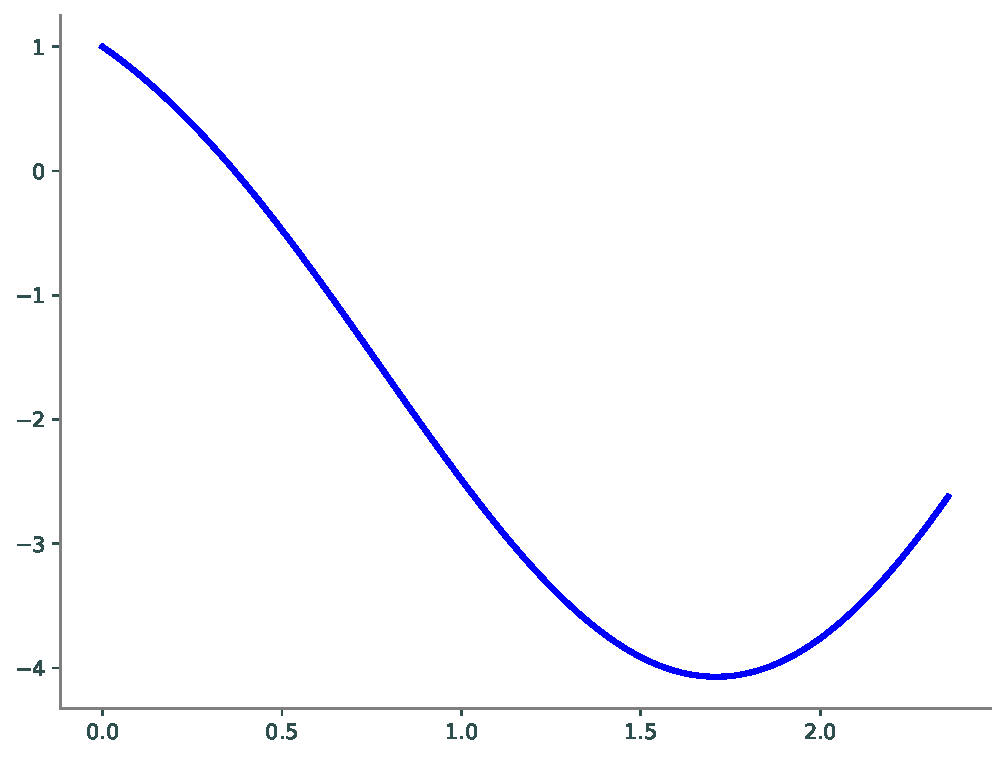
\includegraphics[height=3.5in]{figures/example1.pdf}
\caption{The solution to the BVP \eqref{eq:shooting:bvp1} from the above example.}
\label{fig:shooting:shooting1}
\end{figure}

%\end{comment}

\begin{problem}
\label{prob:shooting:shooting1}
Appropriately defined initial value problems will usually have a unique solution.
Boundary value problems are not so straightforward; they may have no solution or they may have several, and you may have to determine which solutions are physically interesting.

Use the secant method to solve the following BVP:\footnote{This example is from \textit{Numerical Solution of Boundary Value Problems for Ordinary Differential Equations} by Ascher, Mattheij, and Russell, page 89.}
\begin{equation*}
\begin{split}
y'' &= -e^{y-1}, \quad x \in [0,1],\\
y(0) &=y(1) =1.
\end{split}
\end{equation*}
This BVP has two solutions.
Using the secant method, find both numerical solutions and print their initial slopes.
Plot the solutions and compare with Figure \ref{fig:shooting:shooting1}.
What initial values $s_0, s_1$ did you use to find them?
\end{problem}

\begin{figure}[H]
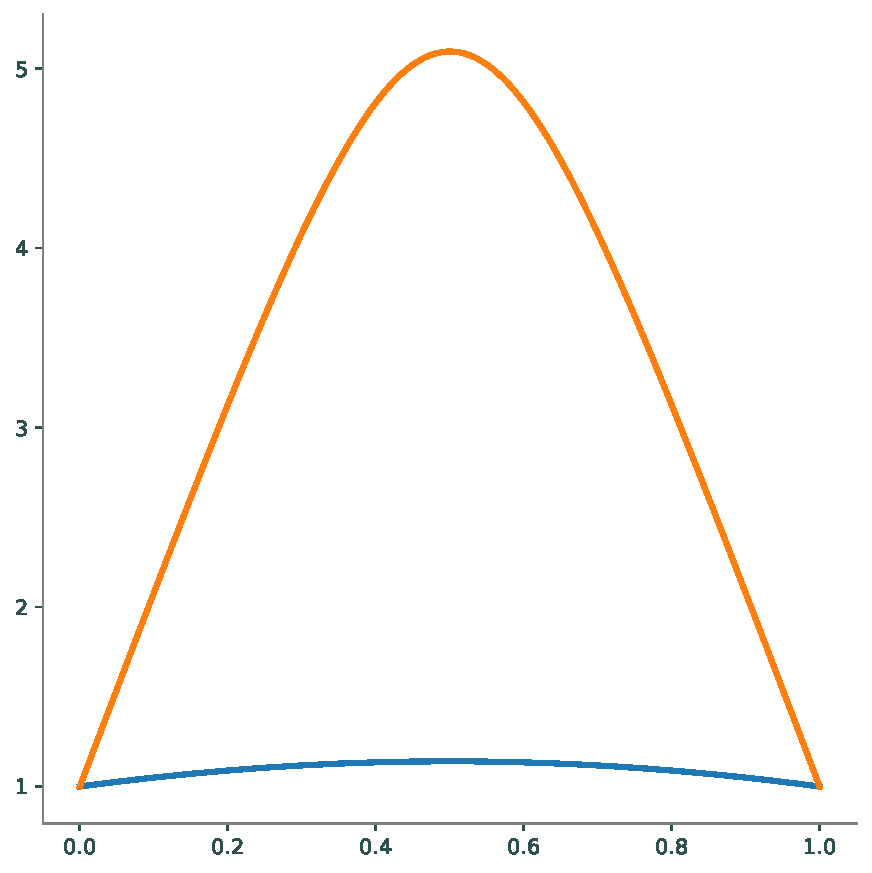
\includegraphics[height=4in]{figures/problem1.pdf}
\caption{Both solutions to the boundary value problem given in Problem \ref{prob:shooting:shooting1}.}
\label{fig:shooting:shooting1}
\end{figure}

Instead of using the secant method, let us consider how to solve for $h'(s)=\frac{\partial }{\partial s} y(b,s)$ for problems of the form given in \eqref{eq:shooting:shooting_bvp}.
For typical systems of ODEs, the solution $y(x,s)$ is smooth enough that it can be differentiated with respect to $x$ and $s$ in any order.\footnote{This is guaranteed to be the case if the right hand side of the ODE is \(C^1\), as in all of the examples here, as this guarantees both partial derivatives of \(y\) are continuous.} % see page 6 of https://sites.math.washington.edu/~burke/crs/555/555_notes/continuity.pdf
Let $z(x,s) = \frac{\partial }{\partial s} y(x,s),$ and note that \(h'(s)=z(b,s)\).
Using the chain rule, we obtain
\begin{eqnarray*}
z'' = \frac{\partial }{\partial s} y''(x,s) &=& \frac{\partial f}{\partial y} (x,y(x,s),y'(x,s)) \cdot \frac{dy}{ds}(x,s) ,\\
&+& \frac{\partial f}{\partial y'} (x,y(x,s),y'(x,s)) \cdot \frac{\partial y'}{\partial s}(x,s),
\end{eqnarray*}
Using the initial conditions associated with $y(x,s)$ and noting that $z(x, s) = \frac{\partial }{\partial s}y(x, s)$ and $z'(x, s) = \frac{\partial }{\partial s}y'(x, s)$, we obtain the following initial value problem for $z(x,s)$:
\begin{eqnarray*}
z'' &=& z\frac{\partial f}{\partial y} (x,y,y') + z' \frac{\partial f}{\partial y'} (x,y,y')
,\quad a \leq x \leq b, \\
 z(a, s) &=& 0,\ z'(a, s) = 1.
\end{eqnarray*}

To use Newton's method, the IVPs for $y$ and $z$ must be solved simultaneously.
The iterative method then becomes
\begin{align}
s_{n+1} &= s_n-\frac{h(s)}{h'(s)}\nonumber
\\
&=s_n - \frac{ y(b,s_n) - \beta}{z(b,s_n)}, \,\, n = 0,1,\hdots \label{eq:shooting:newtonmethod}
\end{align}

We will run through an example to demonstrate this method. Let
\begin{equation*}
\begin{split}
y'' &= 3 + \frac{2y}{x^2}, \,\, x \in [1,e],\\
y(1) &= 6, \\
y(e) &= e^2 + \frac{6}{e},
\end{split}
\end{equation*}
and let $s=y'(1)$. Then
\begin{equation*}
f = y'' = 3 + \frac{2y}{x^2},
\end{equation*}
and
\begin{align*}
\begin{split}
h(s) &= y(b,s) = y(e,s),
\\
h'(s) &= \frac{\partial}{\partial s} y(e,s).
\end{split}
\end{align*}
We then solve iteratively for $s$ using Newton's method, starting with an initial guess $s_0$. With each iteration, we need to solve the initial value problem for $y$ and $z$, given an $s_n$, using the first order system defined by
\begin{align*}
\begin{split}
\begin{bmatrix}y\\y'\\z\\z'\end{bmatrix}'
&= \begin{bmatrix}y'\\3 + \frac{2y}{x^2}
\\z'\\z\frac{\partial f}{\partial y} (x,y,y') + z' \frac{\partial f}{\partial y'} (x,y,y')\end{bmatrix}
= \begin{bmatrix}y'\\3 + \frac{2y}{x^2}
\\z'\\ \frac{2z}{x^2}\end{bmatrix},
\\
z(1,s_n) &= 0, \quad z'(1,s_n) = 1,
\\
y(1,s_n) &= 6, \quad y'(1,s_n) = s_n.
\end{split}
\end{align*}
We then use the solutions for $y(x,s_n)$ and $z(x,s_n)$ to find $s_{n+1}$, using equation \eqref{eq:shooting:newtonmethod}, and iterate.


\begin{problem}
\label{prob:shooting:shooting2}
Use Newton's method to solve the BVP
\begin{equation*}
\begin{split}
y'' &= 3 + \frac{2y}{x^2}, \,\, x \in [1,e],\\
y(1) &= 6, \\
y(e) &= e^2 + \frac{6}{e}.
\end{split}
\end{equation*}
Plot your solution, and compare with Figure \ref{fig:shooting:shooting2}.
What is an appropriate initial guess?

%Hint: Update your ODE function from the previous problem to solve for $y$, $y'$, $z$, $z'$ simultaneously.
%This can be done by first rewriting the equations for $y''$ and $z''$ as a system of first order differential equations.
\end{problem}

\begin{figure}[h]
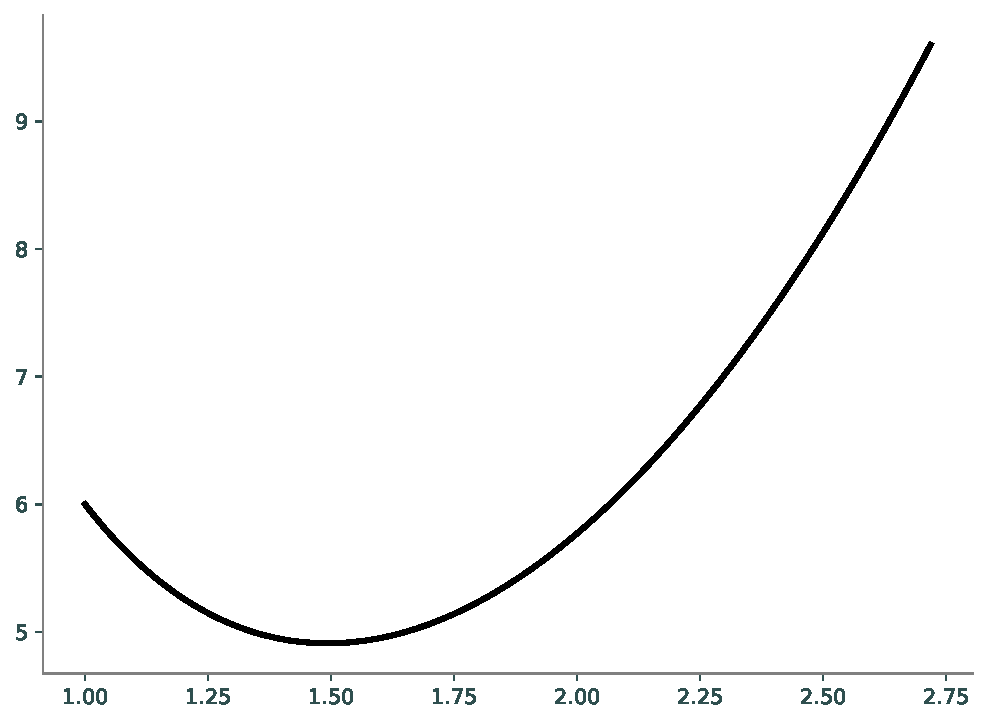
\includegraphics[height=4in]{figures/problem2.pdf}
\caption{The solution of  $y'' = 3 + 2y/x^2,$ satisfying the boundary conditions $y(1) = 6$, $ y(e) =  e^2 + 6/e$, given in Problem \ref{prob:shooting:shooting2}.}
\label{fig:shooting:shooting2}
\end{figure}

\section*{The Cannon Problem}

Consider the problem of aiming a projectile at a given target.
Here we will construct a differential equation that describes the path of the projectile and takes into account air resistance.
We will then use the shooting method to determine the angle at which the projectile should be launched.

Let \(t\) denote time, and the coordinates of the projectile be given by $\mathbf{r}(t) = (x(t), y(t))$.
If $\theta(t)$ represents the angle of the velocity vector from the positive $x$-axis and \(v(t)=\Vert\mathbf{v}(t) \Vert\) represents the speed of the projectile, then we have
\begin{align*}
\dot{x} &= v\cos{\theta},\\
\dot{y} &= v\sin{\theta}.
%x' &= v\cos{\theta},\\
%y' &= v\sin{\theta}.
\end{align*}
Note that each of $x,y,\theta$, and $v$ are functions of $t$, so the dot denotes $\frac{d}{dt}$.
The tangent vector to the path traced by the projectile is the unit vector in the direction of the projectile's velocity, so $\mathbf{T}(t) = ( \cos{\theta}, \sin{\theta} )$.
The unit normal vector $\mathbf{N} (t)$ is given by $\mathbf{N} (t)= ( -\sin{\theta}, \cos{\theta} )$.
Thus the relationship between basis vectors $\mathbf{i}, \mathbf{j}$, and $\mathbf{T(t)}, \mathbf{N}(t)$ is given by
\[
\left[\begin{array}{cc}
\cos{\theta} & \sin{\theta} \\
-\sin{\theta} & \cos{\theta}\end{array}\right]
\left[\begin{array}{c}
\mathbf{i} \\
\mathbf{j}
\end{array}\right]
=
\left[\begin{array}{c}
\mathbf{T(t)} \\
\mathbf{N(t)}
\end{array}\right]\]
Let $F_g$ represent the force on the projectile due to gravity, and $F_d$ represent the force on the projectile due to air resistance. (We assume the air is still.)
From Newton's law we have
\begin{align*}
m \dot{\mathbf{v}} &= F_g + F_d.
%m \vec{v}\ ' &= F_g + F_d.
\end{align*}

The drag equation from fluid dynamics says that the force on the projectile due to air resistance is $k v^2 = (1/2)\rho c_D A v^2$, where $\rho$ is the mass density of air (about $1.225$ $\text{kg}/\text{m}^3$), $v$ is the speed of the projectile, and $A$ is its cross-sectional area.
The drag coefficient $c_D$ is a dimensionless quantity that changes with respect to the shape of the object.
(If we assume our projectile is spherical with a diameter of $.2$ m, then its drag coefficient $c_D \approx 0.47$, its cross-sectional area is $\pi/100$ $ \text{m}^2$, and we obtain $k \approx 0.009$.)

Thus the total force on the shell is
\begin{align}
m \dot{\mathbf{v}} &= -mg \mathbf{j} - kv^2 \mathbf{T},\nonumber \\
%m \vec{v}\ ' &= -mg \vec{j} - kv^2 \vec{T},\nonumber \\
&= -mg( \mathbf{T}\sin{\theta}  + \mathbf{N}\cos{\theta}  ) - kv^2 \mathbf{T},\nonumber\\
&= (-mg \sin{\theta} - k v^2 ) \mathbf{T} - mg \mathbf{N}\cos{\theta} .\label{eqn:TForce1}
\end{align}
From the identity
$\mathbf{v} = ( \dot{x}, \dot{y} ) = ( v \cos{\theta}, v \sin{\theta} )$
%$\vec{v} = \langle x', y' \rangle = \langle v \cos{\theta}, v \sin{\theta} \rangle$
we have
\begin{align}
m \dot{\mathbf{v}} = {} & m( \dot{v} \cos{\theta} - v\dot{\theta}\sin{\theta}  ,\dot{v}\sin{\theta} + v\dot{\theta}\cos{\theta} ) \nonumber \\
= {} & m(\dot{v}\cos{\theta} - v\dot{\theta}\sin{\theta} )(\cos{\theta} \mathbf{T} - \sin{\theta}\mathbf{N}) \nonumber \\
& + m(\dot{v} \sin{\theta} + v\dot{\theta}\cos{\theta} )(\mathbf{T} \sin{\theta}  + \mathbf{N}\cos{\theta} ) ,  \nonumber \\
= {} & m(\mathbf{T}\dot{v} + \mathbf{N}v\dot{\theta}) .\label{eqn:TForce2}
%
%m \vec{v}' = {} & m\langle v' \cos{\theta} - v\sin{\theta} \cdot \theta' ,v'\sin{\theta} + v\cos{\theta} \cdot \theta' \rangle \nonumber \\
%= {} & m(v'\cos{\theta} - v\sin{\theta} \cdot \theta')(\cos{\theta} \vec{T} - \sin{\theta}\vec{N}) \nonumber \\
%& + m(v' \sin{\theta} + v\cos{\theta} \cdot \theta')( \sin{\theta} \vec{T} + \cos{\theta} \vec{N}) ,  \nonumber \\
%= {} & m(\vec{T} \cdot v' + \vec{N} \cdot v \cdot \theta') .\label{eqn:TForce2}
\end{align}
From equations \eqref{eqn:TForce1} and \eqref{eqn:TForce2} we have
\begin{align*}
%m v' &= -mg\sin{\theta} - k v^2,\\
m \dot{v} &= -mg\sin{\theta} - k v^2,\\
mv\dot{\theta} &= -mg \cos{\theta}.
%mv\theta' &= -mg \cos{\theta}.
\end{align*}
Thus we have the system of differential equations
\begin{align}
\dot{x} &= v\cos{\theta}, \nonumber \\
\dot{y} &= v\sin{\theta},\nonumber \\
\dot{v} &= -g\sin{\theta} -  k v^2/m,\nonumber \\
\dot{\theta} &= -g \cos{\theta}/v. \nonumber
%x' &= v\cos{\theta}, \nonumber \\
%y' &= v\sin{\theta},\nonumber \\
%v' &= -g\sin{\theta} -  k v^2/m,\nonumber \\
%\theta' &= -g \cos{\theta}/v. \nonumber
\end{align}

We can actually write this problem to be independent of \(t\), which will make solving it simpler, since we do not know the final time of impact.
If we assume that $t$ is an smooth invertible function of $x$ (that is, $t = t(x)$), then we obtain
\begin{align*}
\frac{dy}{dx} &= \frac{dy}{dt}\frac{dt}{dx} ,\\
&= \frac{dy}{dt} \frac{1}{\frac{dx}{dt}}, \\
&= \frac{v \sin{\theta}}{v\cos{\theta}} = \tan{\theta}.
\end{align*}
We find $\frac{dv}{dx}$ and $\frac{d\theta}{dx}$ in a similar manner.
Thus our system of differential equations becomes
\begin{align}
	\begin{split}
\frac{dy}{dx} &= \tan {\theta} ,\\
\frac{dv}{dx} &= -\frac{g \sin{\theta} + \mu v^2}{v \cos{\theta}},\\
\frac{d\theta}{dx} &= -\frac{g}{v^2}, \label{eqn:cannon_DEs}
	\end{split}
\end{align}
where $\mu = k/m.$
We can now consider \(y,v,\) and \(\theta\) to be functions of \(x\), and \(x\) to be the independent variable.

\begin{problem}
Suppose we have a cannon that fires a projectile at a velocity of $45\text{ m/s}$, and the projectile has a mass of about $60$ kg, so that $\mu = .0003$.
At what angle $\theta(0)$ should it be fired to land at a distance of $195\text{ m}$?
Use the secant method to find initial values for \(\theta\) that give solutions to the following BVP:
\begin{align}
	\label{eqn:cannon_shooting}
	\begin{split}
\frac{dy}{dx} &= \tan {\theta} ,\\
\frac{dv}{dx} &= -\frac{g \sin{\theta} + \mu v^2}{v \cos{\theta}},\\
\frac{d\theta}{dx} &= -\frac{g}{v^2},\\
y(0)&= y(195) = 0,\\
v(0) &= 45 \text{ m/s}
	\end{split}
\end{align}
($g = 9.8067\text{ m/s}^2$.)

There are four angles $\theta(0)$ that produce solutions for this BVP when $\mu = 0.0003$.
However, only two of the angles are physically meaningful for this problem as they lie in $(0, \pi/2)$, while the others lie in $(\pi, 3\pi/2)$ and correspond to the projectile moving from right to left.
Find and plot the two solutions whose angles lie in $(0, \pi/2)$.
Also find the two solutions when $\mu = 0$ (no air resistance), and compare.
Graphs of the solutions are given in Figure \ref{fig:shooting_cannon_comparison2}.

Keep in mind that the unknown initial condition is $\theta(0)$, not $y'(0)$.
What is the appropriate residual function $h(t)$ to apply the secant method to?
\end{problem}

\begin{figure}[H]
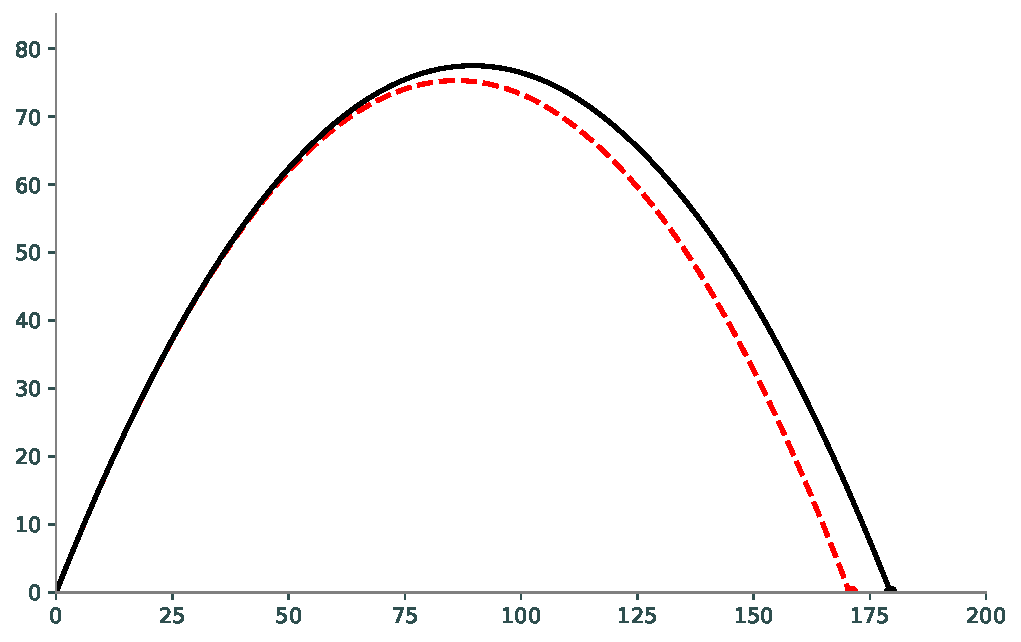
\includegraphics[height=2.5in]{figures/cannon_comparison.pdf}
\caption{Two solutions of the system of equations \eqref{eqn:cannon_DEs}, both with initial conditions  $y(0) = 0 \text{ m}$, $ v(0) = 45 \text{ m/s}$, and $\theta(0)=\pi/3$.
The black curve is the trajectory of a projectile with no air resistance ($\mu = 0$).
The red curve describes the trajectory of a more realistic projectile ($\mu = .0003$).}
\label{fig:shooting_cannon_comparison1}
\end{figure}

\begin{figure}[H]
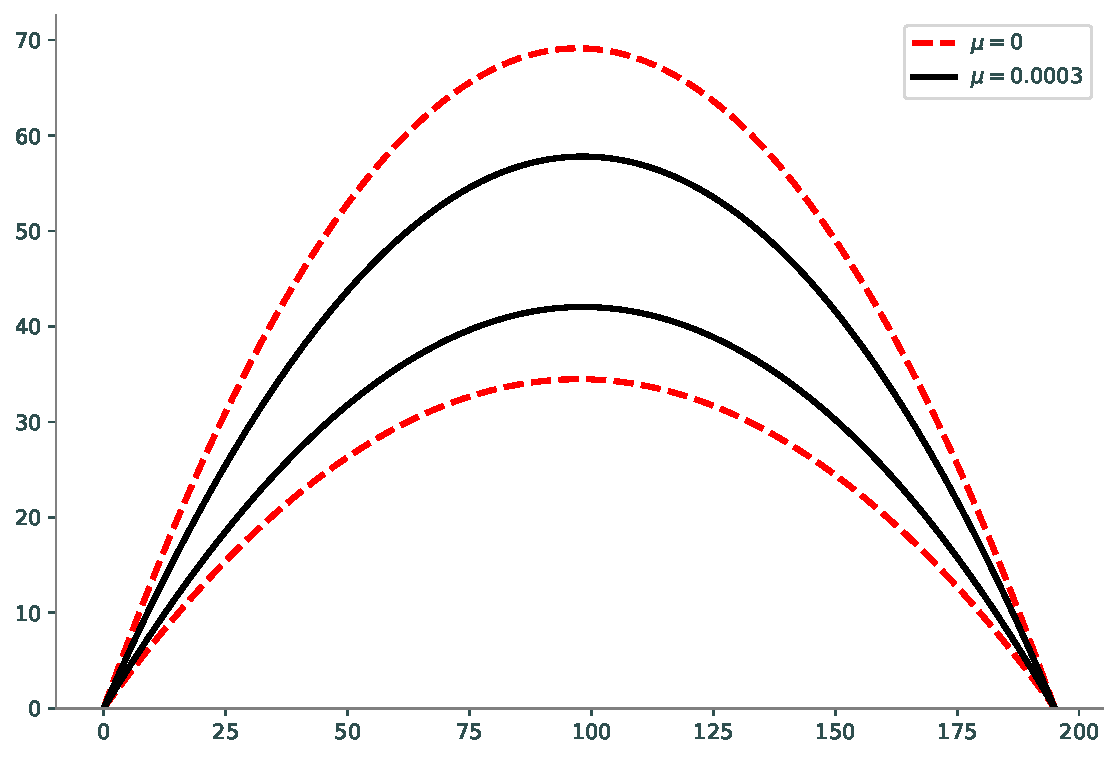
\includegraphics[height=2.5in]{figures/problem3.pdf}
\caption{The two solutions of the boundary value problem \eqref{eqn:cannon_shooting} when the air resistance is described by the parameter $\mu = 0.0003$,
and the two solutions with no air resistance ($\mu = 0$).}
\label{fig:shooting_cannon_comparison2}
\end{figure}
